% Dataset construction (D): three collection rails. (1) Congressional hearings from GovInfo; (2) the independent
% C-SPAN reference; (3) firm disclosures from the SEC 10-K archive. Every number is the measured count reported in
% the D notebooks (D1.1 to D4.1).
% Same visual language as T1.X, T2.X, and T3/TEMP/T3.X. Compile: pdflatex fig_dataset_construction.tex
\documentclass[border=8pt]{standalone}
\usepackage[T1]{fontenc}
\usepackage{tgtermes}
\usepackage{tikz}
\usetikzlibrary{positioning, shapes.symbols, shadows, arrows.meta, fit, backgrounds, calc}

% Figure Style Guide colors (S3)
\definecolor{RED}{HTML}{B31942}
\definecolor{BLUE}{HTML}{0A3161}
\definecolor{MIDNIGHTBLUE}{HTML}{004953}
\definecolor{GREY}{HTML}{A6A6A8}
\definecolor{BLACK}{HTML}{101820}
\colorlet{SUBTEXT}{GREY!35!BLACK}

% second line inside a block: the fact behind the block, in small dark grey
\newcommand{\sub}[1]{\\[2pt]{\scriptsize\color{SUBTEXT}#1}}

\begin{document}
\hyphenpenalty=10000 \exhyphenpenalty=10000
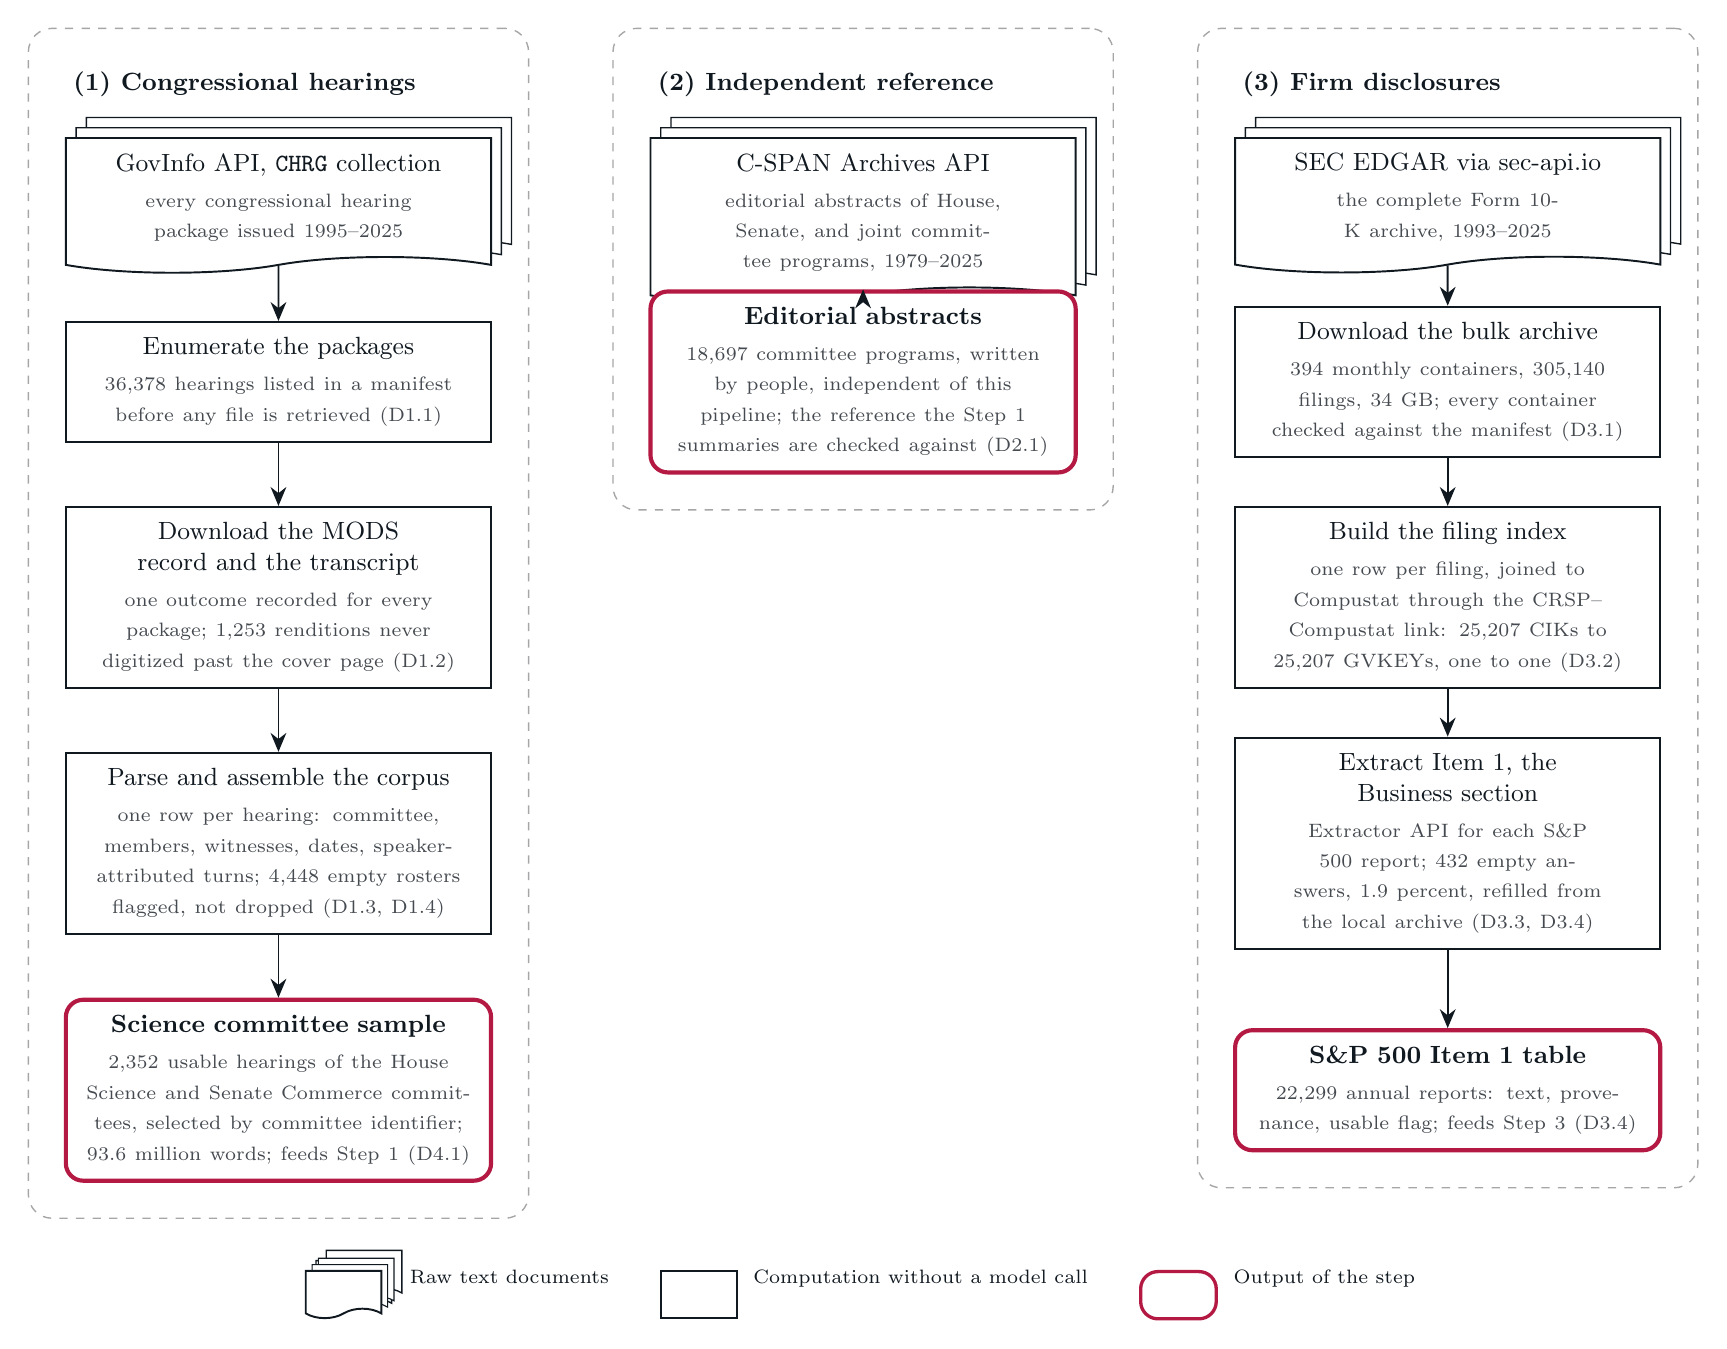
\begin{tikzpicture}[
  font=\small, text=BLACK, color=BLACK,
  node distance=8mm and 14mm,
  every node/.style={align=center},
  flow/.style={-{Stealth[length=2.4mm, width=2mm]}, line width=0.7pt, BLACK},
  % raw text: a stack of documents with a torn lower edge
  rawdoc/.style={tape, tape bend top=none, tape bend height=2mm, draw=BLACK, line width=0.7pt, fill=white,
                 text width=50mm, minimum height=15mm, inner sep=2mm,
                 double copy shadow={shadow xshift=1.3mm, shadow yshift=1.3mm, draw=BLACK, fill=white, line width=0.5pt}},
  % computation without a model call
  compute/.style={rectangle, draw=BLACK, line width=0.7pt, fill=white, text width=50mm, minimum height=13mm, inner sep=2mm},
  % data products of the step
  output/.style={rectangle, rounded corners=2.2mm, draw=RED, line width=1.5pt, fill=white, text width=50mm, minimum height=13mm, inner sep=2mm},
  lane/.style={draw=GREY, line width=0.5pt, dashed, rounded corners=3mm, inner sep=4.5mm},
  lanetitle/.style={font=\small\bfseries, text=BLACK, anchor=south west, inner sep=1mm},
]

% ---------------------------------------------------------------- (1) Congressional hearings
\node[rawdoc] (H1) {GovInfo API, \texttt{CHRG} collection\sub{every congressional hearing package issued 1995--2025}};
\node[compute, below=of H1] (H2) {Enumerate the packages\sub{36,378 hearings listed in a manifest before any file is retrieved (D1.1)}};
\node[compute, below=of H2] (H3) {Download the MODS record and the transcript\sub{one outcome recorded for every package; 1,253 renditions never digitized past the cover page (D1.2)}};
\node[compute, below=of H3] (H4) {Parse and assemble the corpus\sub{one row per hearing: committee, members, witnesses, dates, speaker-attributed turns; 4,448 empty rosters flagged, not dropped (D1.3, D1.4)}};
\node[output, below=of H4] (H5) {\textbf{Science committee sample}\sub{2,352 usable hearings of the House Science and Senate Commerce committees, selected by committee identifier; 93.6 million words; feeds Step 1 (D4.1)}};

% ---------------------------------------------------------------- (2) Independent reference
\node[rawdoc, anchor=north west] (R1) at ([xshift=20mm]H1.north east) {C-SPAN Archives API\sub{editorial abstracts of House, Senate, and joint committee programs, 1979--2025}};
\node[output] (R2) at (H2 -| R1) {\textbf{Editorial abstracts}\sub{18,697 committee programs, written by people, independent of this pipeline; the reference the Step 1 summaries are checked against (D2.1)}};

% ---------------------------------------------------------------- (3) Firm disclosures
\node[rawdoc, anchor=north west] (F1) at ([xshift=20mm]R1.north east) {SEC EDGAR via sec-api.io\sub{the complete Form 10-K archive, 1993--2025}};
\node[compute] (F2) at (H2 -| F1) {Download the bulk archive\sub{394 monthly containers, 305,140 filings, 34 GB; every container checked against the manifest (D3.1)}};
\node[compute] (F3) at (H3 -| F1) {Build the filing index\sub{one row per filing, joined to Compustat through the CRSP--Compustat link: 25,207 CIKs to 25,207 GVKEYs, one to one (D3.2)}};
\node[compute] (F4) at (H4 -| F1) {Extract Item 1, the Business section\sub{Extractor API for each S\&P 500 report; 432 empty answers, 1.9 percent, refilled from the local archive (D3.3, D3.4)}};
\node[output] (F5) at (H5 -| F1) {\textbf{S\&P 500 Item 1 table}\sub{22,299 annual reports: text, provenance, usable flag; feeds Step 3 (D3.4)}};

% ---------------------------------------------------------------- flows
\foreach \a/\b in {H1/H2, H2/H3, H3/H4, H4/H5, R1/R2, F1/F2, F2/F3, F3/F4, F4/F5}
  \draw[flow] (\a) -- (\b);

% ---------------------------------------------------------------- lanes and titles
\node[lanetitle] (titleH) at ([yshift=4mm]H1.north west) {(1) Congressional hearings};
\node[lanetitle] (titleR) at ([yshift=4mm]R1.north west) {(2) Independent reference};
\node[lanetitle] (titleF) at ([yshift=4mm]F1.north west) {(3) Firm disclosures};
\begin{scope}[on background layer]
  \node[lane, fit=(titleH)(H1)(H5)] {};
  \node[lane, fit=(titleR)(R1)(R2)] {};
  \node[lane, fit=(titleF)(F1)(F5)] {};
\end{scope}

% ---------------------------------------------------------------- legend
% One matrix node, anchored on the middle lane's center line, so the legend is centered under the three lanes.
\matrix[anchor=north, inner sep=0pt, column sep=1.2mm, row sep=0pt, nodes={inner xsep=0.8mm}] (legend) at ($(H5.south -| R1)+(0,-11mm)$) {
  \node[rawdoc, text width=8mm, minimum height=6mm, inner sep=0.8mm, tape bend height=1.2mm,
        double copy shadow={shadow xshift=0.8mm, shadow yshift=0.8mm, draw=BLACK, fill=white, line width=0.4pt}] {}; &[1.5mm]
  \node[font=\scriptsize] {Raw text documents}; &[4.5mm]
  \node[compute, text width=8mm, minimum height=6mm, inner sep=0.8mm] {}; &
  \node[font=\scriptsize] {Computation without a model call}; &[4.5mm]
  \node[output, text width=8mm, minimum height=6mm, inner sep=0.8mm, line width=1.2pt] {}; &
  \node[font=\scriptsize] {Output of the step}; \\
};

\end{tikzpicture}
\end{document}
